\chapter{Introduction}

\label{ch:introduction}

This document is designed primarily for visualization purposes, serving as a guide to showcase formatting and structuring. 

Chapter \ref{ch:introduction}, titled "\nameref{ch:introduction}", features one image  and one table. These examples are included to enrich the "List of Figures" and "List of Tables" sections, demonstrating how to effectively incorporate and reference such elements within a document. 

The subsequent chapters contain placeholder text. This example text is intended to illustrate potential content layouts and to further demonstrate text formatting options in a comprehensive manner.

In order to make the reference section visible, we also need some references \cite{liu2017} to display there\cite{jones2017,liu2017}.

\section{Background}

\begin{wrapfigure}{r}{0.5\textwidth}
    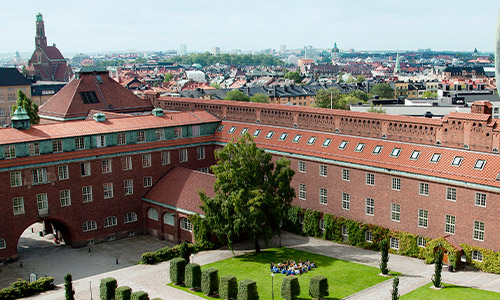
\includegraphics[width=\linewidth]{images/kth-courtyard.jpg}
    \caption{The KTH courtyard is a pretty neat place.}
    \label{fig:kth-courtyard}
\end{wrapfigure}

\lipsum[2]

\section{Problem}

\lipsum[3]

\begin{table}[ht]
    \centering
    \begin{minipage}{\textwidth}
        {\sffamily\textbf{Annual Sales Report}} \\
        {\sffamily{Fiscal Year 2023}} \\
        
        \begin{tabularx}{\textwidth}{ 
            >{\raggedright\arraybackslash}X 
            >{\raggedleft\arraybackslash}X 
            >{\raggedleft\arraybackslash}X 
            >{\raggedleft\arraybackslash}X 
            >{\raggedleft\arraybackslash}X }
            \toprule
            Product & Q1 Sales (\$) & Q2 Sales (\$) & Q3 Sales (\$) & Q4 Sales (\$) \\
            \midrule
            Product A & 25,000 & 27,000 & 24,000 & 29,000 \\
            Product B & 20,000 & 22,500 & 19,000 & 20,000 \\
            \bottomrule
        \end{tabularx}
        
        \caption{Sales numbers for the fiscal year 2023. This description is pretty long and spans over multiple lines.}
        \label{tab:sales-2023}
    \end{minipage}
\end{table}

\noindent\lipsum[4]

\subsection{Purpose and Research Question}

\lipsum[5] % placeholder text